\subsection{Power BI}\label{subsec:power-bi}

Microsoft's take on business intelligence is called Power BI, and it is a powerful tool that can be used to visualize
data from a wide range of sources~\cite{power-bi}.
It differs from~\acrshort{ga4} in that it is not focused on website analytics, but rather on any data it is given.
This can be sales data, user data, or any other data that can be stored in a database.
The main purpose of Power BI is to help businesses make better decisions based on the data they have.
This is very similar to the purpose of this project, as the goal is to help the café owners make better decisions based
on their sales data, as they are currently lacking~\acrlong{bi} tools.
Therefore, Power BI is a good tool to look at for existing solutions on how to visualize the data in a way that is easy
to understand and use.

\begin{figure}[H]
    \centering
    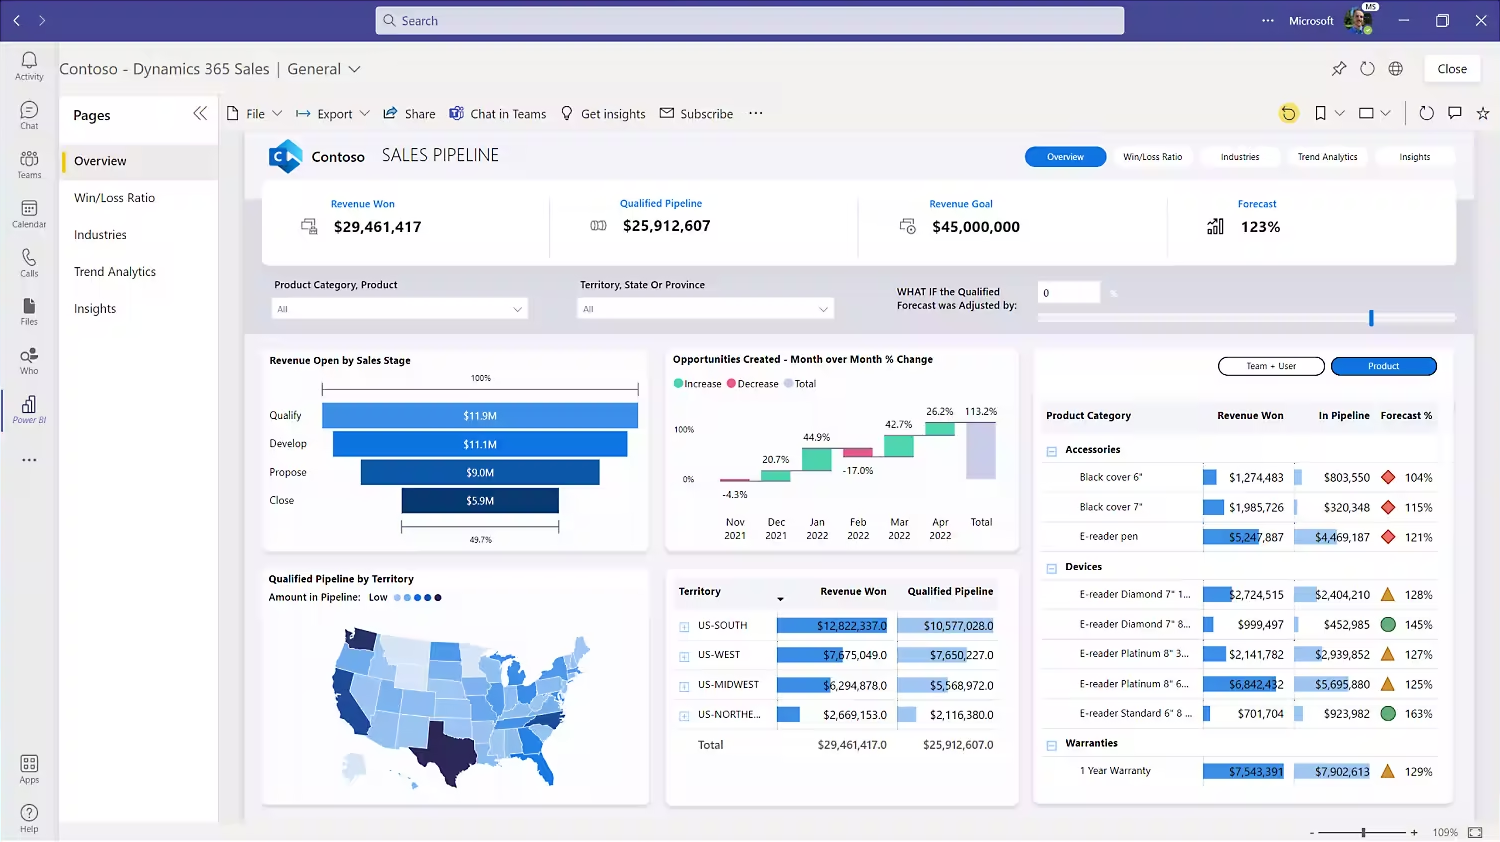
\includegraphics[width=1\textwidth]{PBI-overview}
    \caption{Power BI report example.
    }\label{fig:PBI-overview}
\end{figure}

Power BI is very customizable, so the design, layout and statistics will differ from company to company.
That's what makes Power BI so powerful, as it can be tailored to the specific needs of the company.
It is very similar to Microsoft Excel in that it uses formulas and functions to calculate statistics, and then presents
the data using charts, but it is much more powerful, as it features a wide range of visualizations and data sources.
That data can be dynamic, so it updates in real-time.
The user also has a lot more control over what data is shown and how it is shown.
That data is organized into a report, similar to the one shown in Figure~\ref{fig:PBI-overview}, which can be shared
with other users.
The report is interactive, so the user can click on different parts of the report to see more detailed data or to
filter the data in different ways.

\begin{figure}[H]
    \centering
    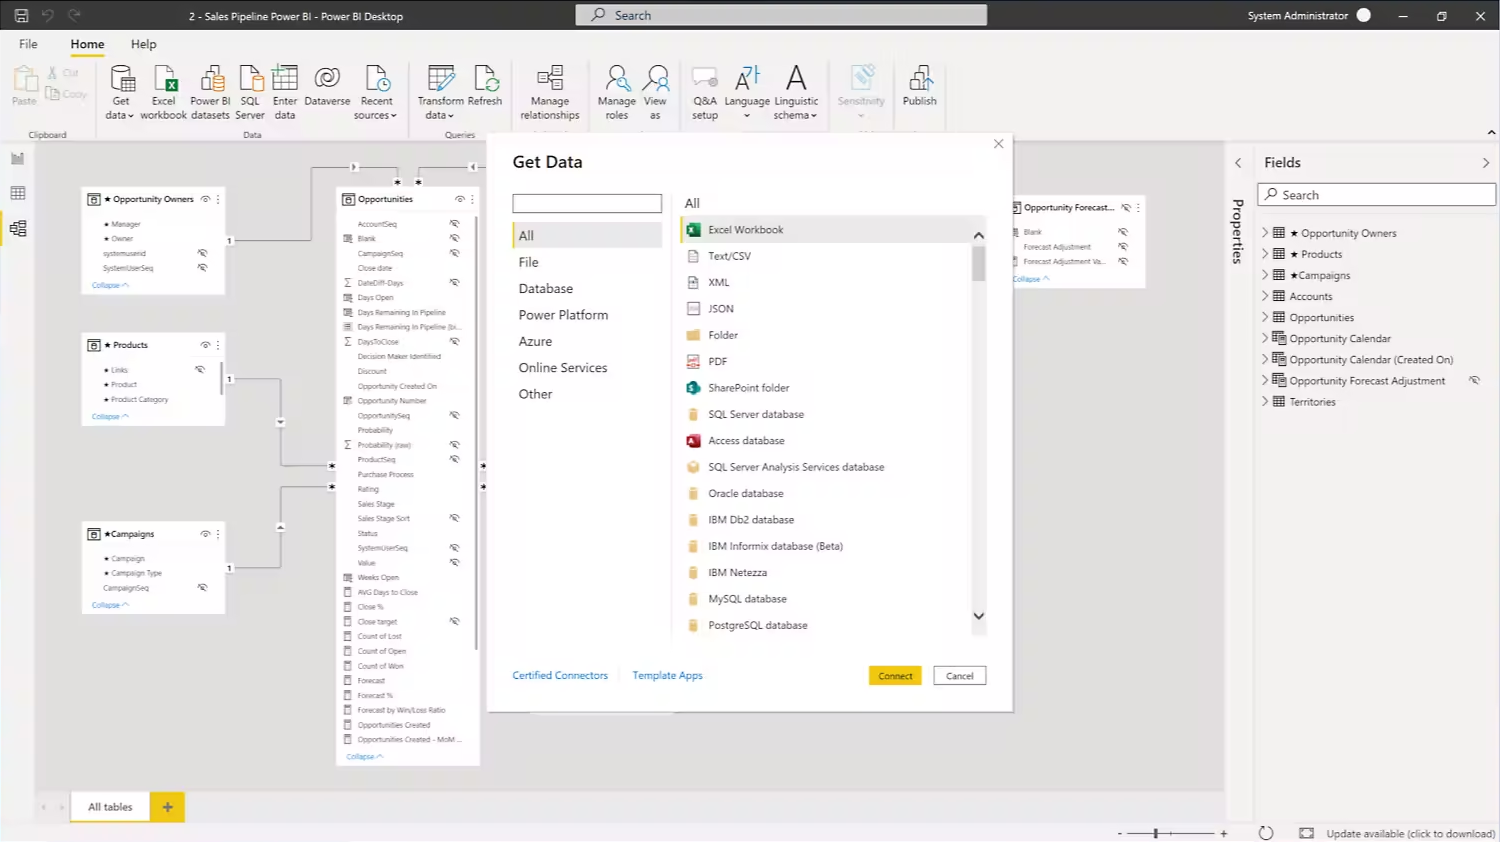
\includegraphics[width=1\textwidth]{PBI-data}
    \caption{Configuring input data in Power BI.\@
    }\label{fig:PBI-data}
\end{figure}

Figure~\ref{fig:PBI-data} shows an example of how the input data can be configured in Power BI~\cite{power-bi}.
The user can choose from a wide range of data sources, such as databases, files, and online services.
The data can then be transformed using Power Query~\cite{power-query}, which is a powerful tool that can be used to
clean, transform, and merge data from different sources.
It is similar to a standard SQL query, but it is specifically designed for Microsoft's tools, such as Power BI.\@
The data can then be visually manipulated using Power BI's drag-and-drop interface, which is very user-friendly and
intuitive.

\begin{figure}[H]
    \centering
    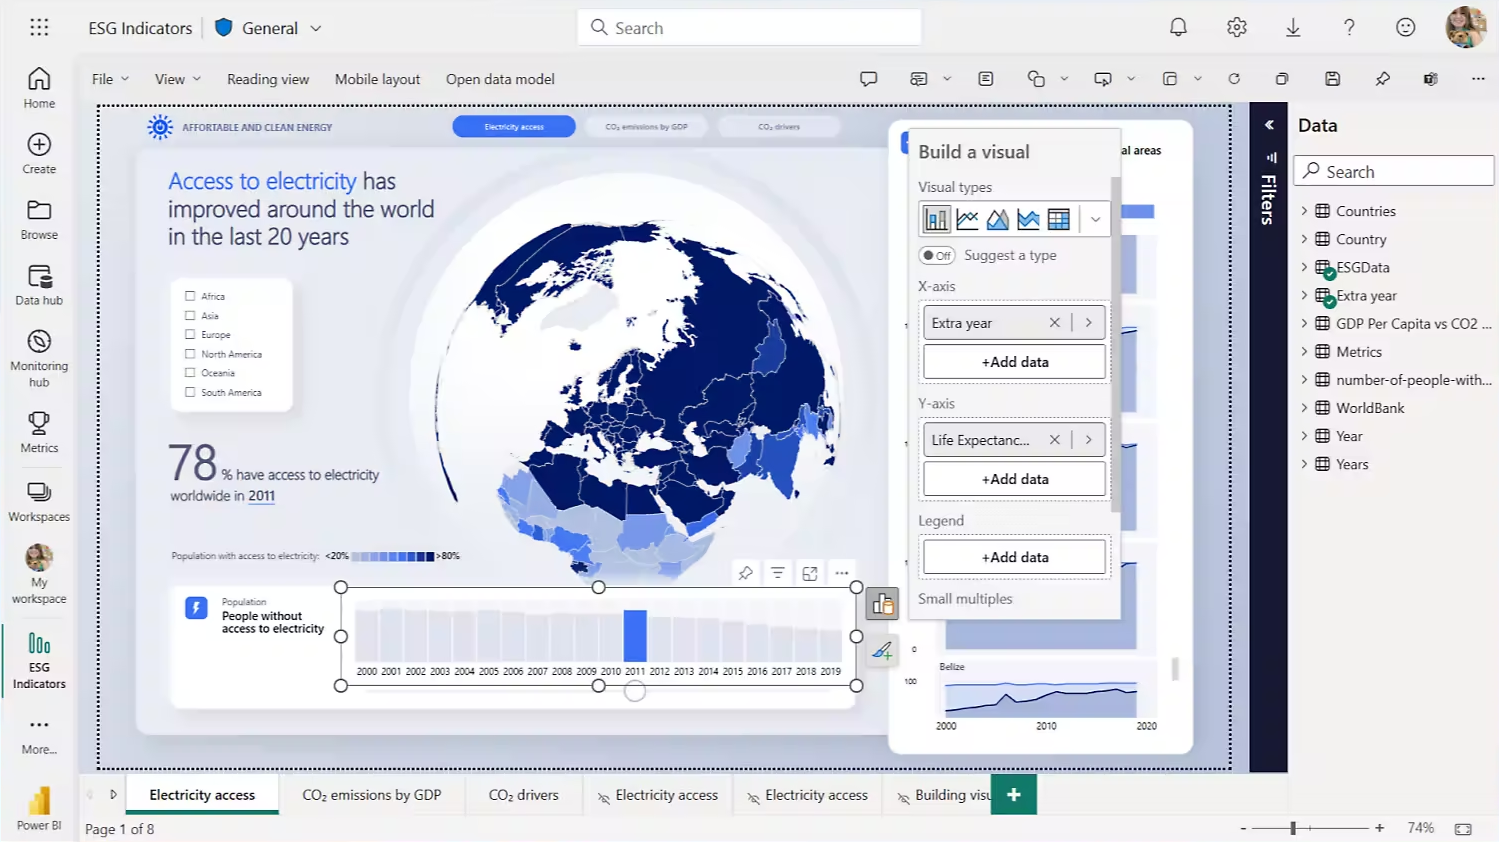
\includegraphics[width=1\textwidth]{PBI-report}
    \caption{Configuring the report in Power BI.\@
    }\label{fig:PBI-report}
\end{figure}

Figure~\ref{fig:PBI-report} shows an example of how the report can be configured in Power BI~\cite{power-bi}.
There is a wide range of visualizations, such as tables, graphs, and maps that the user can pick from.
These visualizations can then be customized in many ways, such as changing the colors, fonts, and sizes.
They are manipulated similar to Microsoft's PowerPoint, where the user can drag and drop elements to change the layout.

While Power BI is a powerful tool, it is not without its disadvantages.
The main disadvantage is that it is not free, as it is a part of Microsoft's Office 365 suite.
There is a free tier, but it is very limited in what it can do, and it is not suitable for commercial use.
And because Power BI is so powerful, it can be overwhelming for new users, as there are so many features and options.
